\documentclass{article}

\usepackage{fontspec}
\setmainfont{Open Sans-Regular}
\usepackage{tikz}
\usetikzlibrary{shapes.gates.logic.US}
\input{dft-tikz}
\definecolor{normalfillcolor}{gray}{0.7}
\setlength\paperwidth{50cm}
\setlength\paperheight{50cm}
\setlength\textheight{50cm}
\setlength\hoffset{-1in}
\newdimen\zigzagvert
\newdimen\gatesize
\gatesize=17mm
\zigzagvert=5mm % Connections first go this far down, then zig-zag to
                % their target.
\pagestyle{empty}

\begin{document}
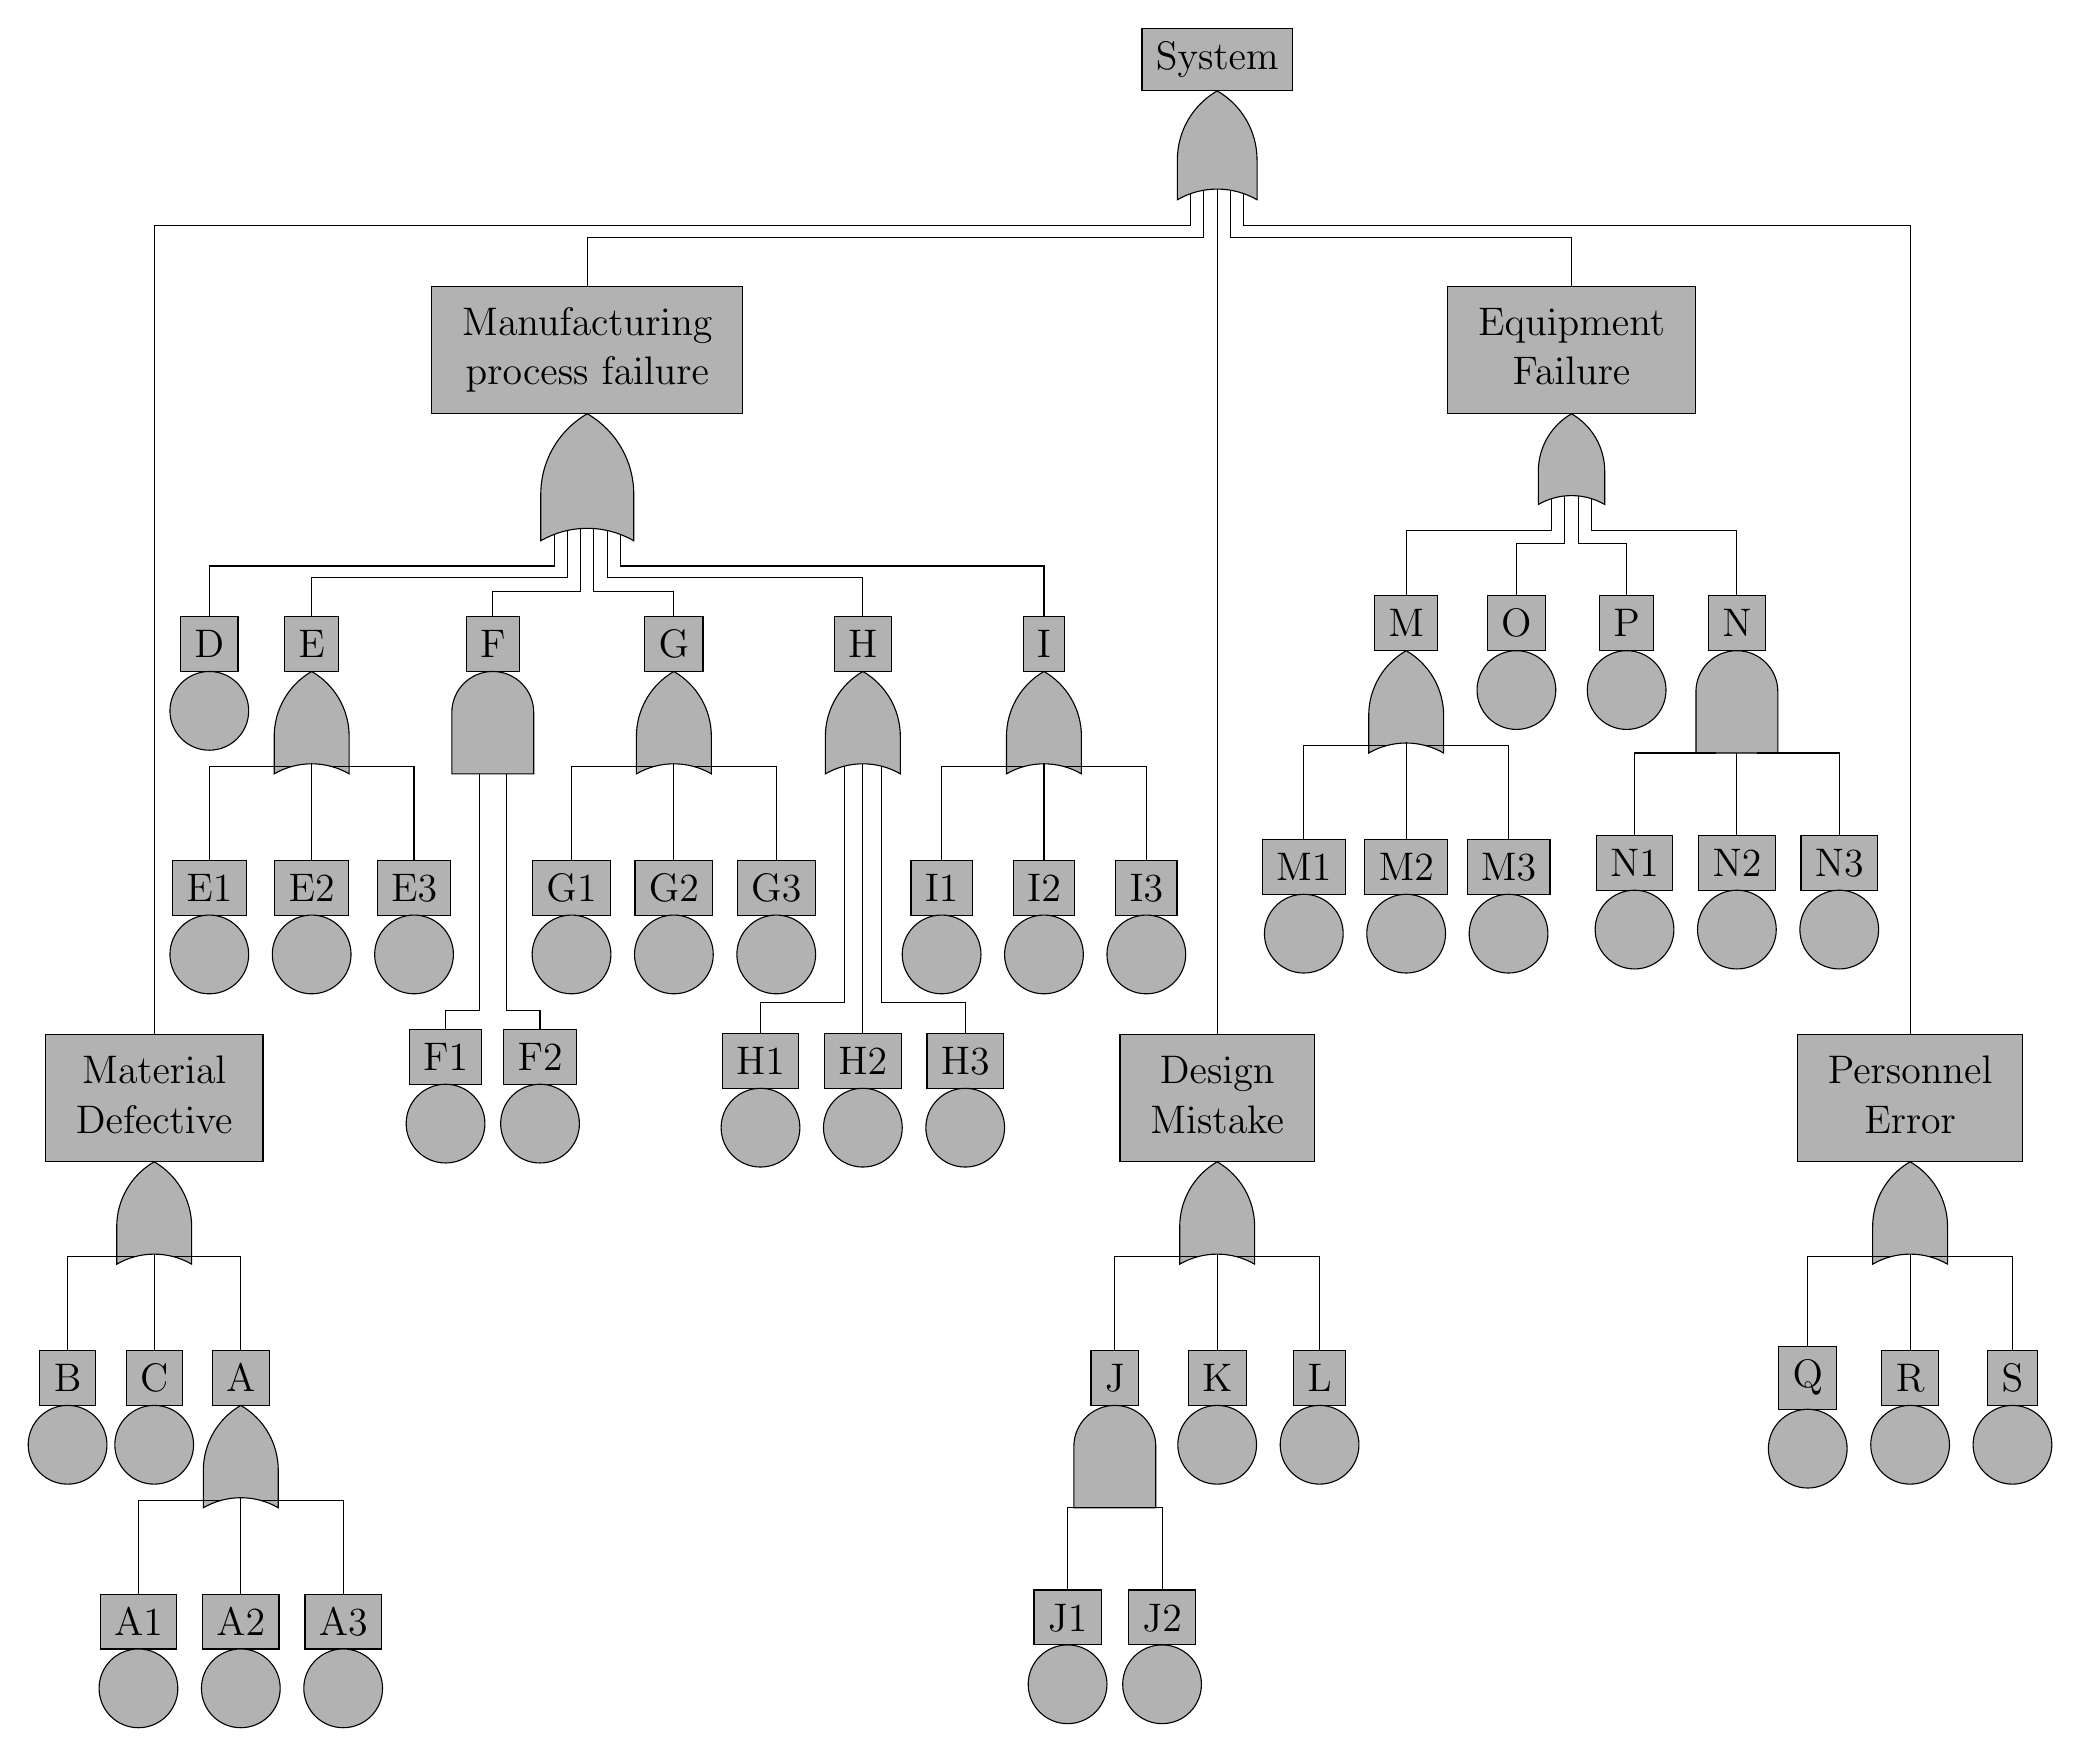
\begin{tikzpicture}[
	rectangle/.style={fill=normalfillcolor, inner sep=5pt},
	node distance=2cm,
	every node/.style={outer sep=0pt,font=\Large},
]
% Input 1 ignored (would be input count).
\def\basicevent#1[#2](#3)#4{
        \node[rectangle, draw, #2, minimum height=5.5mm](#3box){#4};
        \node[circle, minimum width=1cm, fill=normalfillcolor, draw,
		anchor=north] at (#3box.south) (#3) {};
}
% Input 1: Text in triangle.
\def\transferevent#1[#2](#3)#4{
        \node[rectangle, draw, #2, minimum height=5.5mm](#3box){#4};
	\path[draw, fill=normalfillcolor] (#3box.south)
		-- ++(-8mm, -15mm) -- ++(16mm, 0) -- (#3box.south);
	\path (#3box.south) ++ (0, -15mm) node[anchor=south] (#3) {#1};
}
\def\seqevent#1[#2](#3)#4{
        \node[rectangle, draw, #2, minimum height=1cm, minimum width=15mm](#3){};
	\node[anchor=north] at (#3.north) (#3box) {#4};
	\draw[->, line width=1mm] (#3.west) -- (#3.east);
}
\def\orevent#1[#2](#3)#4{
        \node[rectangle, draw, #2, minimum height=5.5mm](#3box){#4};
        \node[or gate US, minimum width=\gatesize, logic gate inputs=#1, rotate=90, fill=normalfillcolor, draw, anchor=output] at (#3box.south) (#3) {};
}
\def\smallerorevent#1[#2](#3)#4{
        \node[rectangle, draw, #2, minimum height=5.5mm](#3box){#4};
        \node[or gate US, minimum width=13mm, logic gate inputs=#1, rotate=90, fill=normalfillcolor, draw, anchor=output] at (#3box.south) (#3) {};
}
\def\andevent#1[#2](#3)#4{
        \node[rectangle, draw, #2, minimum height=5.5mm](#3box){#4};
        \node[and gate US, minimum width=13mm, logic gate inputs=#1, rotate=90, fill=normalfillcolor, draw, anchor=output] at (#3box.south) (#3) {};
}
% Input 1: Blank for normal, M for mirrored.
\def\sparegate#1[#2](#3)#4{
        \node[spare#1, fill=normalfillcolor, draw, anchor=north, #2]
		(#3) {};
	\node[anchor=north] at (#3.north) (#3box) {#4};
}
% Input 1 ignored (for consistency).
\def\fdepgate#1[#2](#3)#4{
        \node[fdep, fill=normalfillcolor, draw, anchor=north, #2]
		(#3) {};
	\node[anchor=north] at (#3.north) (#3box) {#4};
}
% \connectZZ{G.input}{vert. distance}{child}.
% Draw a line from G.input down by 'vert. distance', then zig-zag to
% child.
\def\connectcust#1#2#3{
	\draw[-] (#1) -- ++(0,#2) -| (#3box);
}
% \connect{G.input}{child} (Note: Only for vertical connections).
\def\connect#1#2{
	\connectcust{#1}{-\zigzagvert}{#2};
}
	\orevent{nnnnn}[](top){System}
	\smallerorevent{nnn}[below of=top, xshift=-135mm, yshift=-10cm](I){\begin{tabular}{c}
		Material\\Defective\end{tabular}}
	\orevent{nnnnnn}[below of=top, xshift=-8cm, yshift=-5mm](II){\begin{tabular}{c}
		Manufacturing\\process failure\end{tabular}}
	\smallerorevent{nnn}[below of=top, xshift=0cm, yshift=-10cm](III){\begin{tabular}{c}
		Design\\Mistake\end{tabular}}
	\orevent{nnnn}[below of=top, xshift=45mm, yshift=-5mm](IV){\begin{tabular}{c}
		Equipment\\Failure\end{tabular}}
	\smallerorevent{nnn}[below of=top, xshift=88mm, yshift=-10cm](V){\begin{tabular}{c}
		Personnel\\Error\end{tabular}}
	\connectcust{top.input 1}{-4mm}{I}
	\connectcust{top.input 2}{-6mm}{II}
	\connect{top.input 3}{III}
	\connectcust{top.input 4}{-6mm}{IV}
	\connectcust{top.input 5}{-4mm}{V}
	\smallerorevent{nnn}[below of=I, xshift=11mm](A){A}
	\basicevent [below of=I, xshift=-11mm](B){B}
	\basicevent [below of=I, xshift=0pt](C){C}
	\connect{I.input 3}{A}
	\connect{I.input 1}{B}
	\connect{I.input 2}{C}
	\basicevent [below of=A, xshift=-13mm](A1){A1}
	\basicevent [below of=A, xshift=0cm](A2){A2}
	\basicevent [below of=A, xshift=13mm](A3){A3}
	\connect{A.input 1}{A1}
	\connect{A.input 2}{A2}
	\connect{A.input 3}{A3}
	\basicevent [below of=II, xshift=-48mm](D){D}
	\smallerorevent{nnn}[below of=II, xshift=-35mm](E){E}
	\andevent{nn}[below of=II, xshift=-12mm](F){F}
	\smallerorevent{nnn}[below of=II, xshift=11mm](G){G}
	\smallerorevent{nnn}[below of=II, xshift=35mm](H){H}
	\smallerorevent{nnn}[below of=II, xshift=58mm](I){I}
	\connectcust{II.input 1}{-4mm}{D}
	\connectcust{II.input 2}{-6mm}{E}
	\connectcust{II.input 3}{-8mm}{F}
	\connectcust{II.input 4}{-8mm}{G}
	\connectcust{II.input 5}{-6mm}{H}
	\connectcust{II.input 6}{-4mm}{I}
	\basicevent [below of=E, xshift=-13mm](E1){E1}
	\basicevent [below of=E, xshift=0cm](E2){E2}
	\basicevent [below of=E, xshift=13mm](E3){E3}
	\connect{E.input 1}{E1}
	\connect{E.input 2}{E2}
	\connect{E.input 3}{E3}
	\basicevent [below of=F, yshift=-22mm, xshift=-6mm](F1){F1}
	\basicevent [below of=F, yshift=-22mm, xshift=6mm](F2){F2}
	\connectcust{F.input 1}{-3cm}{F1}
	\connectcust{F.input 2}{-3cm}{F2}
	\basicevent [below of=G, xshift=-13mm](G1){G1}
	\basicevent [below of=G, xshift=0cm](G2){G2}
	\basicevent [below of=G, xshift=13mm](G3){G3}
	\connect{G.input 1}{G1}
	\connect{G.input 2}{G2}
	\connect{G.input 3}{G3}
	\basicevent [below of=H, yshift=-22mm, xshift=-13mm](H1){H1}
	\basicevent [below of=H, yshift=-22mm, xshift=0cm](H2){H2}
	\basicevent [below of=H, yshift=-22mm, xshift=13mm](H3){H3}
	\connectcust{H.input 1}{-3cm}{H1}
	\connectcust{H.input 2}{-3cm}{H2}
	\connectcust{H.input 3}{-3cm}{H3}
	\basicevent [below of=I, xshift=-13mm](I1){I1}
	\basicevent [below of=I, xshift=0cm](I2){I2}
	\basicevent [below of=I, xshift=13mm](I3){I3}
	\connect{I.input 1}{I1}
	\connect{I.input 2}{I2}
	\connect{I.input 3}{I3}
	\andevent{nn}[below of=III, xshift=-13mm](J){J}
	\basicevent [below of=III, xshift=0cm](K){K}
	\basicevent [below of=III, xshift=13mm](L){L}
	\connect{III.input 1}{J}
	\connect{III.input 2}{K}
	\connect{III.input 3}{L}
	\basicevent [below of=J, xshift=-6mm](J1){J1}
	\basicevent [below of=J, xshift=6mm](J2){J2}
	\connect{J.input 1}{J1}
	\connect{J.input 2}{J2}
	\smallerorevent{nnn}[below of=IV, xshift=-21mm](M){M}
	\andevent{nnn}[below of=IV, xshift=21mm](N){N}
	\basicevent [below of=IV, xshift=-7mm](O){O}
	\basicevent [below of=IV, xshift=7mm](P){P}
	\connectcust{IV.input 1}{-4mm}{M}
	\connectcust{IV.input 4}{-4mm}{N}
	\connectcust{IV.input 2}{-6mm}{O}
	\connectcust{IV.input 3}{-6mm}{P}
	\basicevent [below of=M, xshift=-13mm](M1){M1}
	\basicevent [below of=M, xshift=0cm](M2){M2}
	\basicevent [below of=M, xshift=13mm](M3){M3}
	\connect{M.input 1}{M1}
	\connect{M.input 2}{M2}
	\connect{M.input 3}{M3}
	\basicevent [below of=N, xshift=-13mm](N1){N1}
	\basicevent [below of=N, xshift=0cm](N2){N2}
	\basicevent [below of=N, xshift=13mm](N3){N3}
	\connect{N.input 1}{N1}
	\connect{N.input 2}{N2}
	\connect{N.input 3}{N3}
	\basicevent [below of=V, xshift=-13mm](V1){Q}
	\basicevent [below of=V, xshift=0cm](V2){R}
	\basicevent [below of=V, xshift=13mm](V3){S}
	\connect{V.input 1}{V1}
	\connect{V.input 2}{V2}
	\connect{V.input 3}{V3}
\end{tikzpicture}
\end{document}
